\section{Results}\label{sec:results}

\inbrief{Ninth on the final leaderboard at a verified mean proxy of 0.9974, 31.6\%
below RePlAce and 4.9\% above the winner, in a listed 12 minutes per design. Most of our
improvement came from lower congestion, and in the development records the fastest
pipeline also scored best.}

\subsection{Competition result}\label{sec:competition}

Our entry ranked ninth on the final leaderboard (verified mean proxy 0.9974; the
organizers report 132 verified eligible submissions), with zero overlaps and
per-design scores from 0.7829 to 1.2602 (\cref{tab:competition,fig:result-context};
\official). That is 31.6\% below the published RePlAce baseline
\citep{cheng2025updated} and 4.9\% above the winner; ranks four to nine lie within
1.4\% of one another. The listed 12 minutes per design is a fifth of the allowed
hour; among top-ten entries that list a runtime, only Vibe (516\,s) lists a shorter
one, on its own hardware. Before the 20 May resubmission, the leaderboard listed our
13 May entry (v1) at 1.0771; that earlier figure is not a verified result.

\begin{table}[htbp]
\centering
\footnotesize
\caption{Official, final leaderboard (14 August 2026). Mean proxy cost over the 17 IBM designs; lower is better. The organizers report 132 verified eligible submissions. Runtimes are as listed by each entrant on its own hardware; the last column is the change relative to the RePlAce mean.}
\label{tab:competition}
\begin{tabular}{clrrr}
\toprule
Rank & Entry & Mean proxy & Listed runtime & vs RePlAce \\
\midrule
1 & Archgen & 0.9507 & --- & $-34.8\%$ \\
2 & Carrotato & 0.9522 & $\sim$12.4\,min per design & $-34.7\%$ \\
\textbf{\boldmath 9} & \textbf{\boldmath Thinkorplace} & \textbf{\boldmath 0.9974} & \textbf{\boldmath 12\,min per design} & \textbf{\boldmath $-31.6\%$} \\
--- & RePlAce baseline & 1.4578 & --- & --- \\
--- & SA baseline & 2.1251 & --- & $+45.8\%$ \\
\bottomrule
\end{tabular}
\end{table}


\subsection{Where the gain came from}\label{sec:gain}

Three development records cover all 17 designs (\historical); the rest of this
section names them by their mean proxy. The \emph{v1 record} (1.05750) is a 17 May
run of a later variant of the serial v1 pipeline, not the 13 May entry. The
\emph{early single-pipeline record} (1.00835) is a 20 May run of an early version of
the single pipeline. The \emph{0.98199 record} is a 20 May run of the single-pipeline
version from which the ranked entry descends. They differ in code, hardware, budget
and concurrency, so they trace a trajectory rather than isolate causes. All three
beat both published baselines on every design, by 14--46\% against RePlAce
(Appendix~\ref{app:records}).

From the v1 record to the 0.98199 record the mean fell by 7.14\%, and
16 of 17 designs improved. The decrease of 0.07551 splits into 0.00294 from
wirelength, 0.00878 from weighted density and 0.06379 from weighted congestion, so
congestion supplied 84.5\% of the gain (\cref{fig:components}). That is where the
score lives: weighted congestion is 64.8--66.2\% of the mean proxy in each record.
The one regression, IBM02, shows the tradeoff of \cref{fig:placement-tradeoff}:
density fell, but wirelength and congestion rose (total 1.00659 to 1.01265). The
decomposition says which terms moved, not which code change moved them; the smooth
stage gained Gaussian density and the routing trace over the same period, and no
controlled ablation separates them.

\begin{figure}[tbp]
\centering
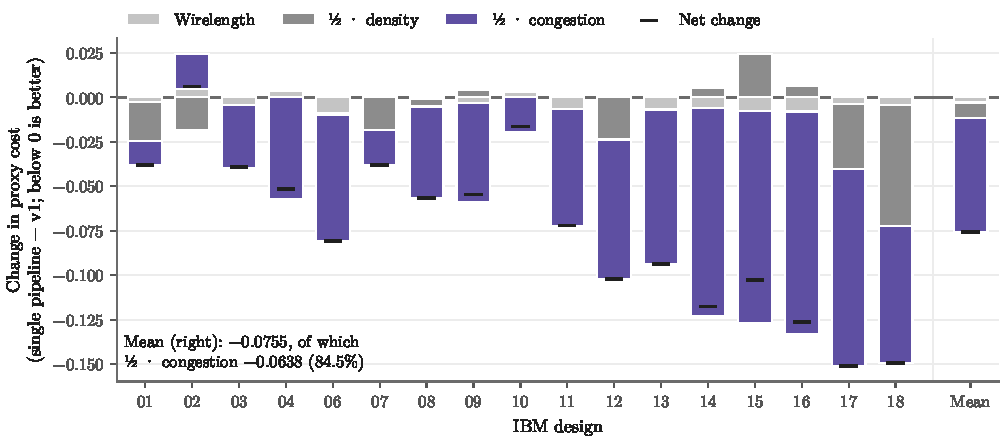
\includegraphics{figures/component_deltas.pdf}
\caption{Change in each weighted score component per design, from the v1 record to the
0.98199 record (20 May, single pipeline; \historical); bars below zero are
improvements, and congestion supplies 84.5\% of the mean decrease. The records are
unmatched in hardware, budget and concurrency.}
\label{fig:components}
\end{figure}

\subsection{A simpler, faster pipeline scored better}\label{sec:simpler}

The v1 record spent 3,192\,s per design on two initializers, three kinds of local
search and a curvature cascade; the early single-pipeline record spent 697\,s; and
the 0.98199 record spent 524\,s, a sixth of v1's time, and scored 7.1\% lower
(\historical). The ranked configuration descends from that pipeline; its official
score and this \historical{} record ran on different hardware with different settings
and are not compared here.

The geometry of \cref{sec:problem} suggests why: exact local search stays near the
arrangement it starts from (\cref{sec:cd}), so more of it mostly refines that
arrangement, while a better smooth start changes the arrangement itself. Only a
matched-compute comparison can test this reading.
